\documentclass[tikz,border=8pt]{standalone}
\usepackage{amsmath,amssymb}
\usetikzlibrary{arrows.meta,calc}

\begin{document}
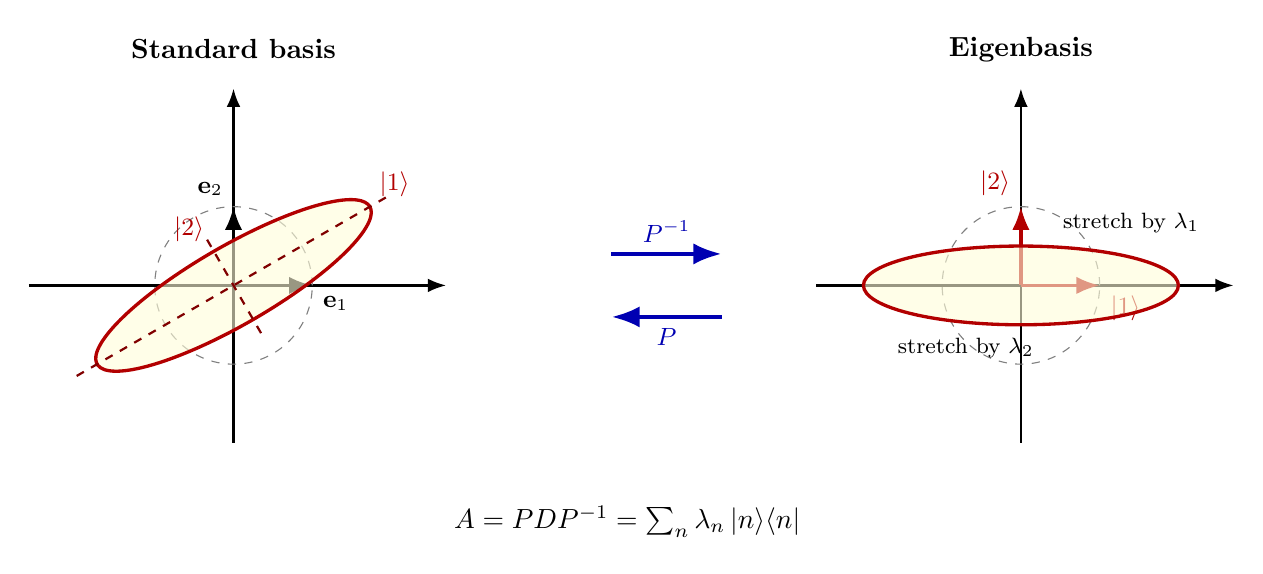
\begin{tikzpicture}[>=Latex, scale=1.0]

  % LEFT — standard basis, A acts on unit circle -> tilted ellipse
  \begin{scope}[xshift=0cm]
    \node[font=\bfseries] at (0, 3.0) {Standard basis};
    \draw[->, thick] (-2.6, 0) -- (2.7, 0);
    \draw[->, thick] (0, -2.0) -- (0, 2.5);

    % standard basis vectors
    \draw[->, very thick, black] (0, 0) -- (1, 0) node[below right, font=\small]{$\mathbf e_1$};
    \draw[->, very thick, black] (0, 0) -- (0, 1) node[above left, font=\small]{$\mathbf e_2$};

    % unit circle
    \draw[thin, gray, dashed] (0, 0) circle (1.0);

    % tilted ellipse: λ1=2, λ2=0.5 along directions at 30°
    \draw[very thick, red!70!black, fill=yellow!15, fill opacity=0.6, smooth, samples=80, domain=0:360]
      plot ({2.0*cos(\x)*cos(30) - 0.5*sin(\x)*sin(30)}, {2.0*cos(\x)*sin(30) + 0.5*sin(\x)*cos(30)});

    % eigenvector axes (dashed)
    \draw[dashed, thick, red!50!black] ({-2.3*cos(30)}, {-2.3*sin(30)}) -- ({2.3*cos(30)}, {2.3*sin(30)});
    \draw[dashed, thick, red!50!black] ({0.7*sin(30)}, {-0.7*cos(30)}) -- ({-0.7*sin(30)}, {0.7*cos(30)});

    \node[red!70!black, font=\small, anchor=south west] at ({2.0*cos(30)}, {2.0*sin(30)}) {$|1\rangle$};
    \node[red!70!black, font=\small, anchor=south east] at ({-0.5*sin(30)}, {0.5*cos(30)}) {$|2\rangle$};
  \end{scope}

  % MIDDLE — transformation arrows
  \begin{scope}[xshift=5.5cm, yshift=0.0cm]
    \draw[->, ultra thick, blue!70!black] (-0.7, 0.4) -- (0.7, 0.4) node[midway, above, font=\small]{$P^{-1}$};
    \draw[<-, ultra thick, blue!70!black] (-0.7, -0.4) -- (0.7, -0.4) node[midway, below, font=\small]{$P$};
  \end{scope}

  % RIGHT — eigenbasis: ellipse axis-aligned
  \begin{scope}[xshift=10cm]
    \node[font=\bfseries] at (0, 3.0) {Eigenbasis};
    \draw[->, thick] (-2.6, 0) -- (2.7, 0);
    \draw[->, thick] (0, -2.0) -- (0, 2.5);

    % eigenbasis vectors (red)
    \draw[->, very thick, red!70!black] (0, 0) -- (1, 0) node[below right, font=\small]{$|1\rangle$};
    \draw[->, very thick, red!70!black] (0, 0) -- (0, 1) node[above left, font=\small]{$|2\rangle$};

    % unit circle
    \draw[thin, gray, dashed] (0, 0) circle (1.0);

    % axis-aligned ellipse
    \draw[very thick, red!70!black, fill=yellow!15, fill opacity=0.6] (0, 0) ellipse (2.0 and 0.5);

    \node[font=\footnotesize, anchor=south] at (1.4, 0.55) {stretch by $\lambda_1$};
    \node[font=\footnotesize, anchor=north] at (-0.7, -0.55) {stretch by $\lambda_2$};
  \end{scope}

  % BOTTOM formula
  \node[align=center, font=\normalsize] at (5, -3.0)
    {$A=PDP^{-1}=\sum_n\lambda_n\,|n\rangle\langle n|$};
\end{tikzpicture}
\end{document}
